\documentclass[book.tex]{subfiles}
\begin{document}
\section{Source Code}
The game engine source code was released on July 21st, 1995. Twenty years later it is still there on id software's ftp\footnote{Transfer File Protocol (along with Finger where J.C.Carmack used to blog) was commonly used in the 90s in the blessed time where you did not have to encrypt everything on the wire.}:\\ 
\\\codeword{ftp://ftp.idsoftware.com/idstuff/source/wolfsrc.zip}.\\
\\
\bu{Trivia :} Before the times of nmap, WireShark and various eavesdropping techniques, FTP\footnote{File Transfer Protocol} was commonly used to transfer files: It was simple and naively transmitted username and password in clear. Needless to say it did not age well...\\

\section{First Contact}
The file \codeword{woldsrc.zip} contains an other self-extracting PKZIP archive. It was a convenience back in the day but it is not practical nowadays. You can deflate it with:\\
\\\codeword{unzip WOLFSRC.1}.\\
\par
A few quick stats:\\

\begin{verbatim}
wolfsrc\$ cloc-1.64.pl .

      96 text files.
      94 unique files.                              
      27 files ignored.

---------------------------------------------------------------------
Language           files          blank        comment           code
---------------------------------------------------------------------
C++                   26           5750           6201          21169
C/C++ Header          42            802            660           3900
Assembly              10            669            732           2150
DOS Batch              1              1              0              4
---------------------------------------------------------------------
SUM:                  79           7222           7593          27223
---------------------------------------------------------------------
\end{verbatim}

Twenty seven thousands lines of code. By 2016 standard it is very little. The game is written 90\% in C.\\


 \begin{fancyquotes}
   We didn't have spell checkers in our editors back then, and I always had poor spelling.  The word "collumn" appears in the source code dozens of times.  After I released the source code, one of the emails that stands out in memory read:
 \bigskip \\
It's "COLUMN", you dumb @\#\$\% !\\
 \bigskip \\
\textbf{John Carmack - Programmer}
 \end{fancyquotes}
 
The archive actually contains more than just \codeword{.H} (headers) and \codeword{.C} (code) files. Also present are:
\begin{itemize}
\item \codeword{GOODSTUF.TXT:} Two emails from fans demonstrating the success of the game: An ex-POW and a Microsoft employee.
\item \codeword{.ASM:} Assembly routines to optimize 3D renderer. Also contains low level routines for I/O.
\item \codeword{SIGNON.OBJ:} The startup screen showing the system characteristic (RAM, EMS, XMS, Joystick, SoundCards) was linked in the binary. The reason why is given later.
\item \codeword{GAMEPAL.OBJ:} Game palette. Hardcoded and linked in the executable for the same reason described previously.
\item \codeword{README:} How to build. You can also find a complete tutorial in the Annexe of this book.
\item Many files resulting from a previous compilation attempt.
\end{itemize}







\section{The Big Picture}
The engine can be divided in three blocks:
\begin{itemize}
\item The 2D renderer let the user set the game.
\item The 3D renderer where most of the time is spent in the game.
\item The sound system which always run concurrently with either 2D or 3D renderer. 
\end{itemize}

\par
\begin{figure}[H]
\centering
 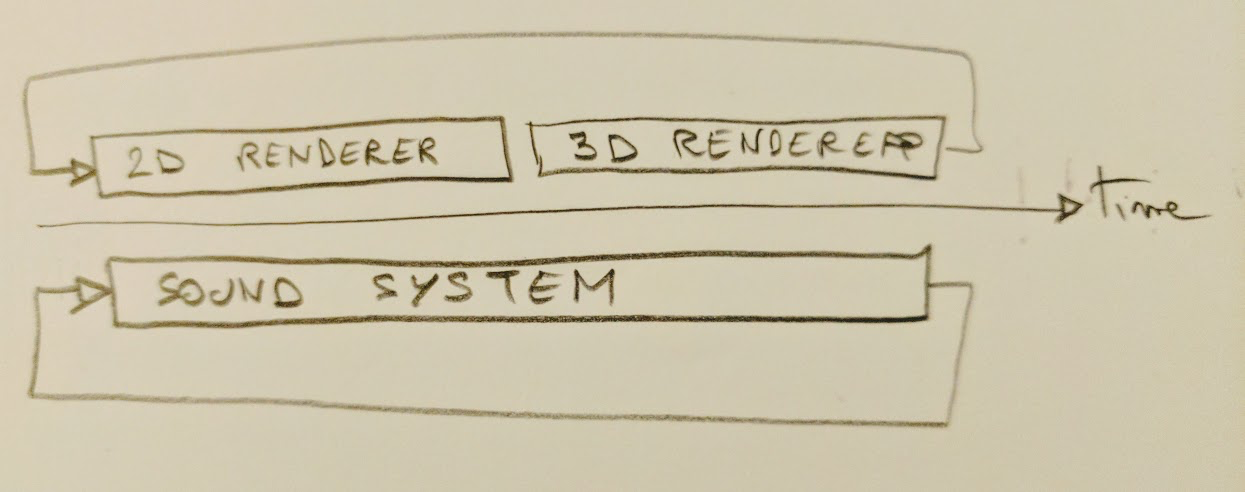
\includegraphics[width=\textwidth]{imgs/three_systems.png}
 \end{figure}
 \par

 
These three systems are amply described in the next sections. The most interesting one is of course the 3D renderer. It is in fact not really 3D: Maps are actually two dimensional designed with square blocks.: e.g, the first level E1M1:\par
\begin{figure}[H]
  \centering
 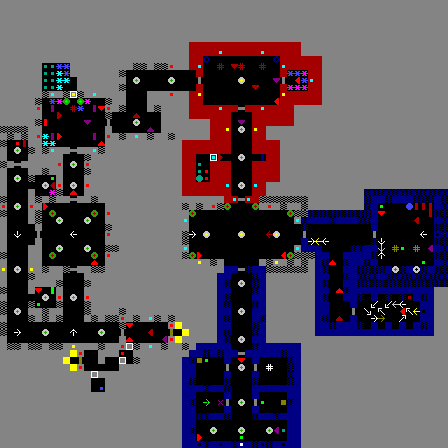
\includegraphics[width=\textwidth]{imgs/e1m1.png}
 \caption{The legendary E1M1 viewed from the top as in TED5 (Player is the green arrow at the bottom).}
\end{figure}
\par 
A 3D dimensional view is faked at runtime:

\begin{figure}[H]
  \centering
 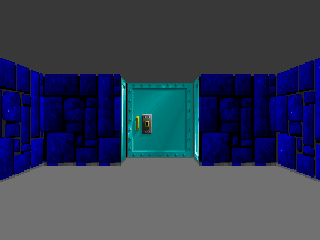
\includegraphics[width=\textwidth]{imgs/ray_caster_explained/beginning.png}
 \caption{As it is rendered at runtime in pseudo-3D from the player point of view.} 
\end{figure}

 The pseudo 3D is generated via a system of raycasting\footnote{Not to be confused with raytracing.}. The previous screenshot being 320 wide by 200 tall, it requested to cast 320 rays (one for each column of wall):

\begin{figure}[H]
  \centering
  
\includegraphics[width=\textwidth]{imgs/ray_caster_explained/beginning.pdf}
 \caption{Complex scene: 320 ray cast.} 
\end{figure}

Raycasting is a powerful even with (for 1991) complex scene.
\begin{figure}[H]
  \centering
 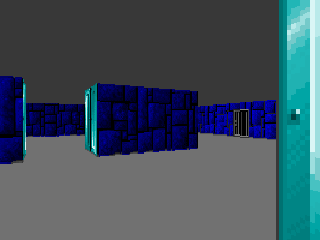
\includegraphics[width=\textwidth]{imgs/ray_caster_explained/out_door.png}
 \caption{Complex scene: rendition.} 
\end{figure}
\par
\begin{figure}[H]
\centering
 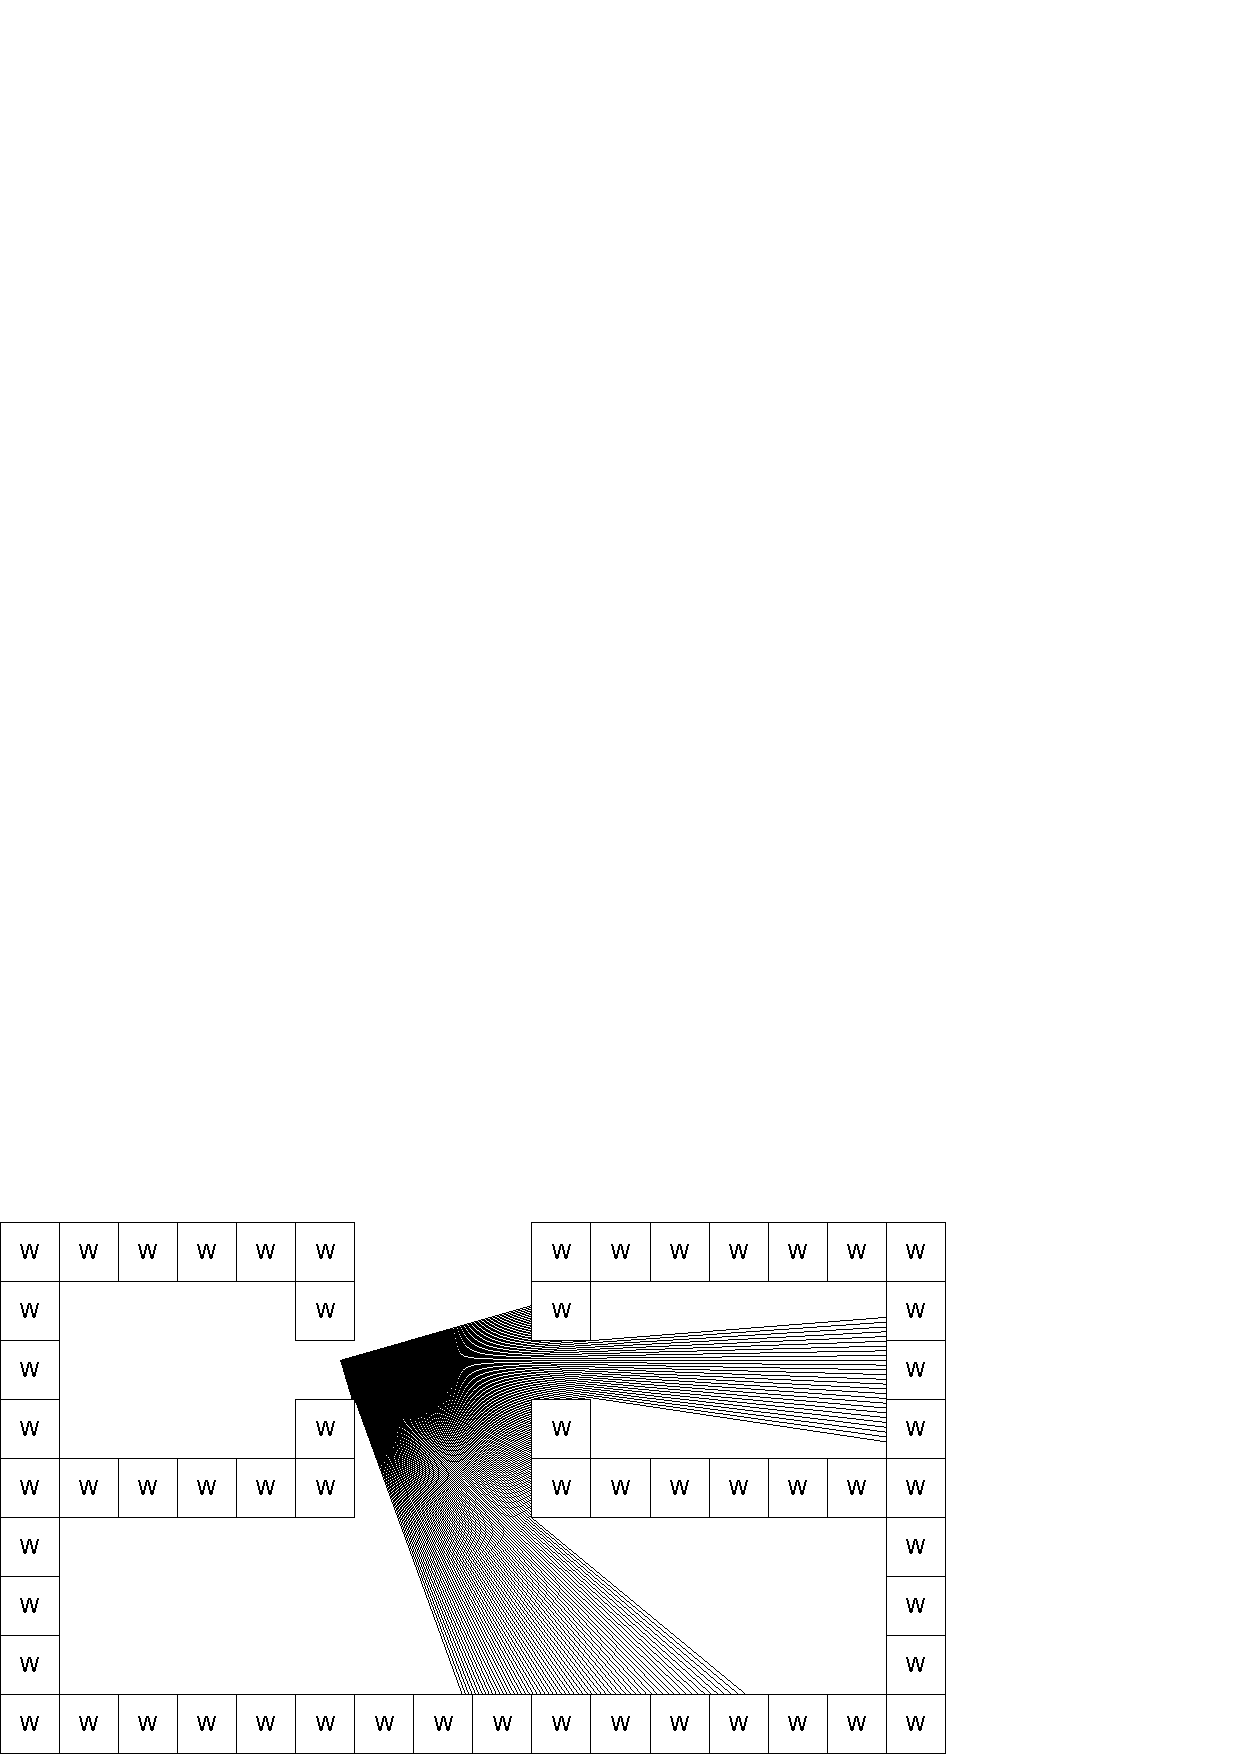
\includegraphics[width=\textwidth]{imgs/ray_caster_explained/out_room.pdf}
 \caption{The 320 rays cast to render the walls in the previous scene.} \label{fig:Raycasting2}
\end{figure}


\subsection{Unrolled loop}
A quick overview of the engine code lets us see the two renderers (the sound system is interrupt driven and therefore is out of the loop).\\
\par
The main function is very simple:\\
\par
\begin{minipage}{\textwidth}
\lstinputlisting[language=C]{code/unrolled_loop_main.c}
\end{minipage}
\par

\cw{Trivia:} Because the game is using Real Mode, C types don't mean what people would expect from a 32 bits system: 
\begin{itemize}
\item \cw{int} and \cw{word} are 16 bits.
\item \cw{long} and \cw{dword} are 32 bits.
\end{itemize}
\par
The engine starts up (all managers are described later):\\
\par
\begin{minipage}{\textwidth}
\lstinputlisting[language=C]{code/unrolled_loop_init.c}
\end{minipage}
\par
The core loop where 2D renderer and 3D renderer are called for ever:\\
\par
\begin{minipage}{\textwidth}
\lstinputlisting[language=C]{code/unrolled_loop_demoloop.c}
\end{minipage}
\par
The play loop which is the 3D renderer. Pretty standard so far:\\
\par
\begin{minipage}{\textwidth}
\lstinputlisting[language=C]{code/unrolled_loop_playloop.c}
\end{minipage}
\par
The sound system which is not in a loop. Instead it is associated with Interrupt XX and called at a regular time interval:\\
\par
\begin{minipage}{\textwidth}
\lstinputlisting[language=C]{code/soundsystem_interrupt.c}
\end{minipage}
\par

















\section{Architecture}

The engine is made of WL\_* files which relies on ID\_* sub-systems called Managers:
\begin{itemize}
	\item Memory
	\item Page
	\item Video
	\item Cache
	\item Sound
	\item User
	\item Input
\end{itemize}
The WL stuff was written specifically for Wolf3D while the ID\_ managers were taken from previous game (Catacomb 3D) and improved for the needs of the new engine.

\begin{figure}[H]
\centering
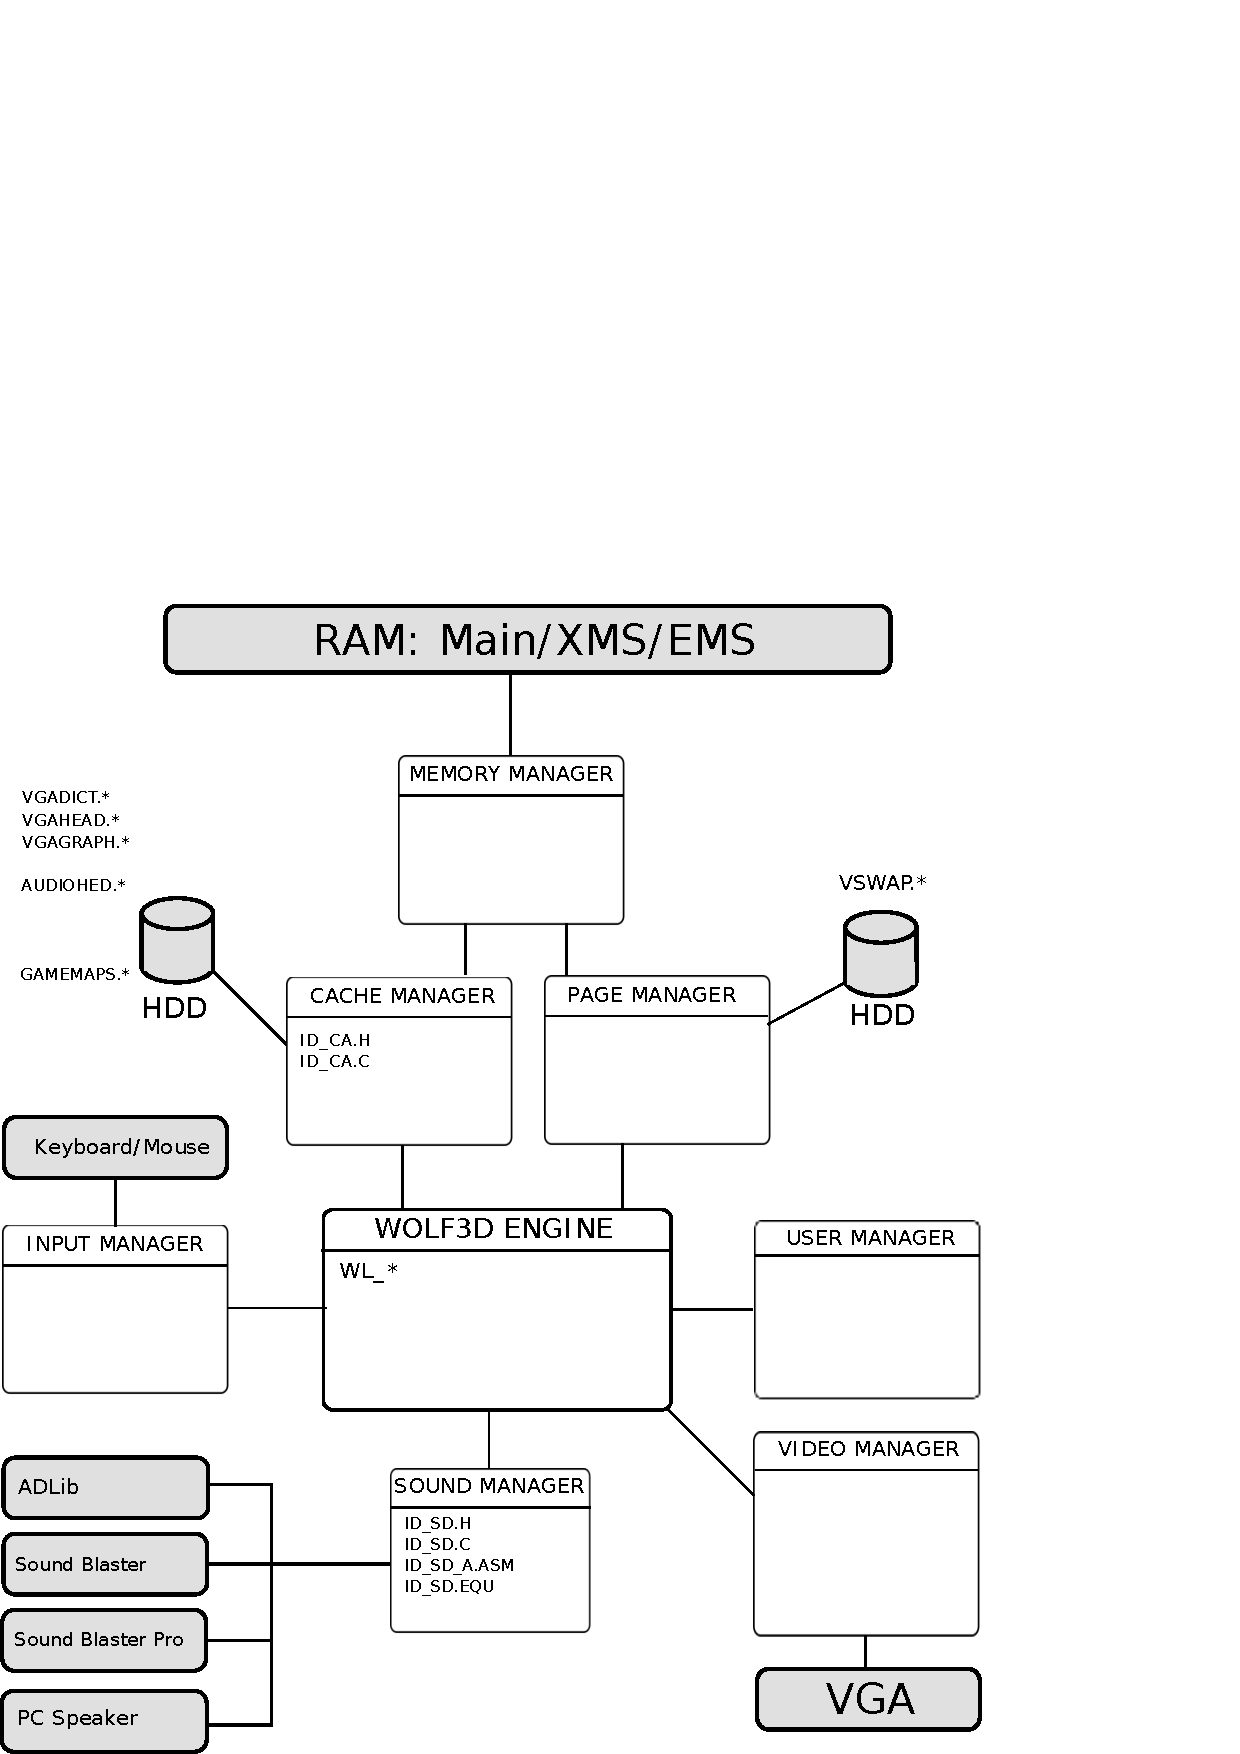
\includegraphics[width=\textwidth]{imgs/architecture.pdf}
\caption{Architecture with engine and sub-systems (in white) connected to I/O (in gray).}
\label{fig:architecture}
\end{figure}
Next to the hard drives (HDD) you can see the assets packed as described in the Team chapter.










\subsection{Memory Manager (MM)}
The engine does not rely on \cw{malloc} to manage memory because it can lead to fragmented memory and no way to compact free space. A linked list keep track of the RAM, dividing it in blocks. A block
point to a starting point in RAM and has a size:\\
 \par
\lstinputlisting[language=C]{code/mm_block.c}
 \par
A block can be marked with attributes:
\begin{itemize}
\item \cw{LOCKBIT} : This block of RAM cannot be moved during garbage collection.
\item \cw{PURGEBITS} : 0-3 level, 0= unpurgable, 3= purge first.
\end{itemize}

The memory manager starts by allocating all available RAM via \cw{malloc} and creates a \cw{LOCKED} block of size 1KB at the end. The linked list uses two pointers: \cw{HEAD} and \cw{ROVER} (for the tail).
 \par
\begin{figure}[H]
\centering
 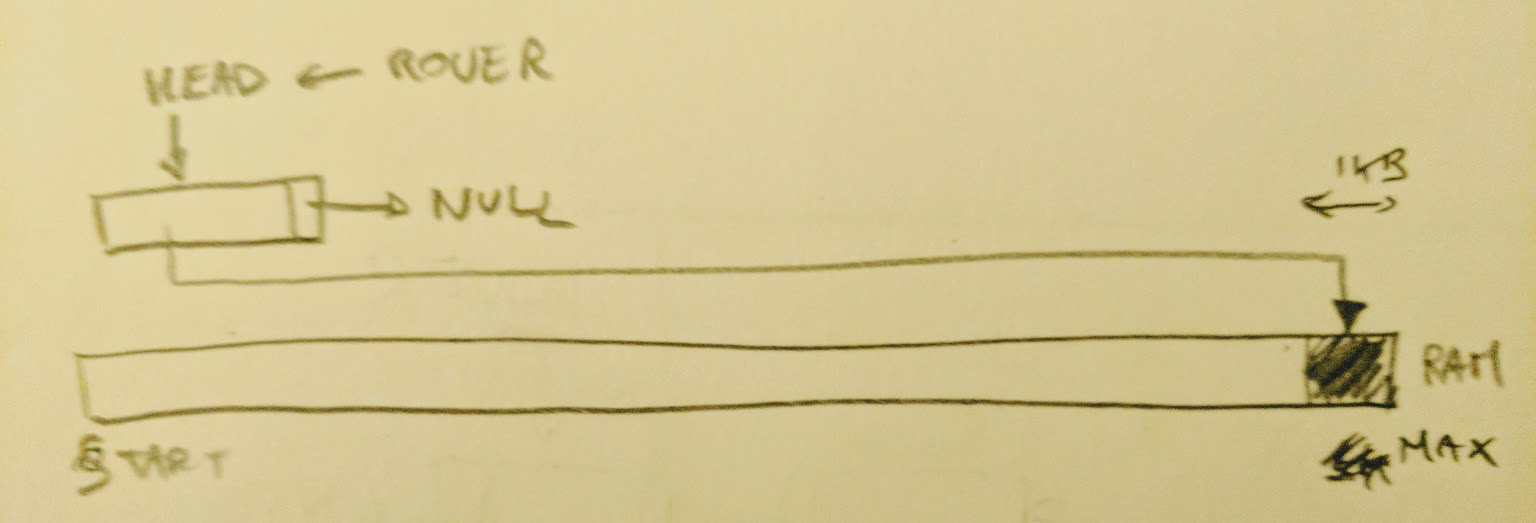
\includegraphics[width=\textwidth]{imgs/mm_start.png}
 \end{figure}
 \par
 The engine interacts with the Memory Manager by requesting RAM (\cw{MM\_GetPtr}) and freeing RAM (\cw{MM\_FreePtr}). To allocate ram , the manager searches for "holes" in the layout. It take up to three passes of increasing complexity. The easier case is when there is enough space after the rover. A new node is added to the linked list and rover moves forward:\\
  \par
\begin{figure}[H]
\centering
 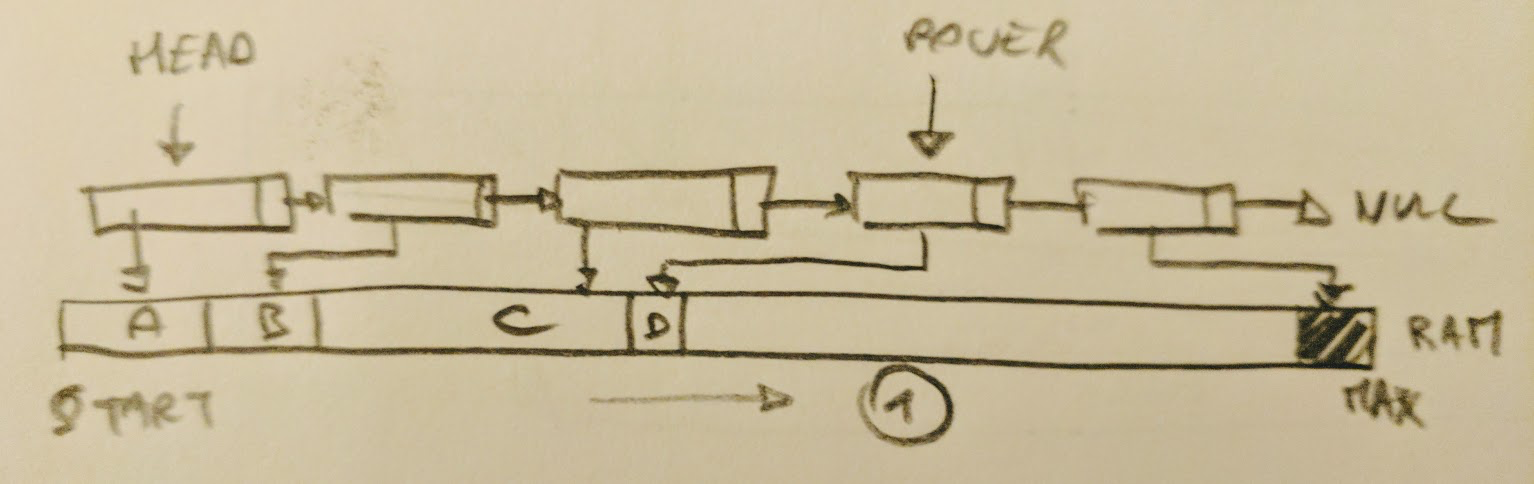
\includegraphics[width=\textwidth]{imgs/mm_after_rover.png}
 \end{figure}
 \par
 If the first pass fails, the second pass looks for a "hole" between the head and the rover:\\
  \par
\begin{figure}[H]
\centering
 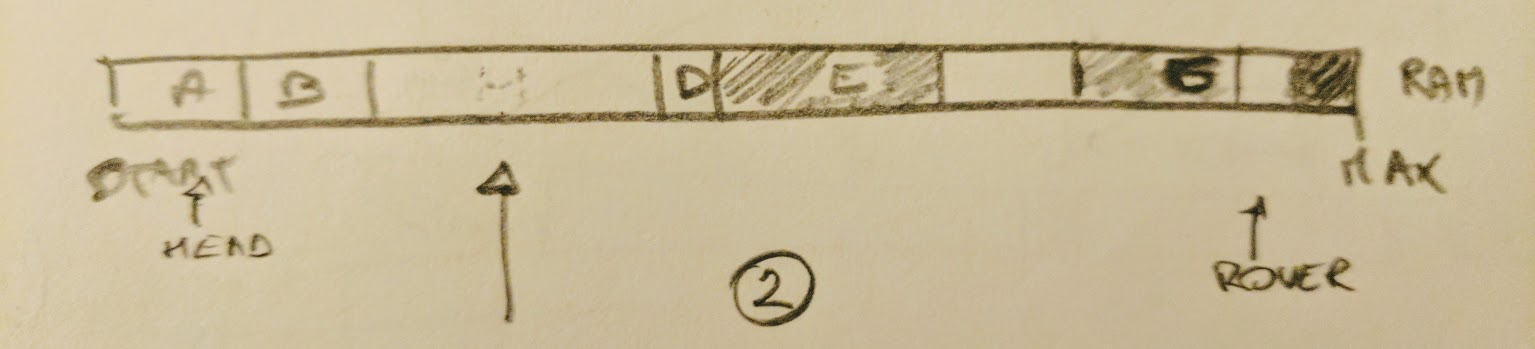
\includegraphics[width=\textwidth]{imgs/mm_before_rover.png}
 \end{figure}
 \par
 In the third pass, it looks like there is nowhere a continuous block of memory big enough to satisfy the request. The manager is going to iterate through the entire linked list and do two things: Delete blocks marked as purgeable and compact the RAM.
  \par
\begin{figure}[H]
\centering
 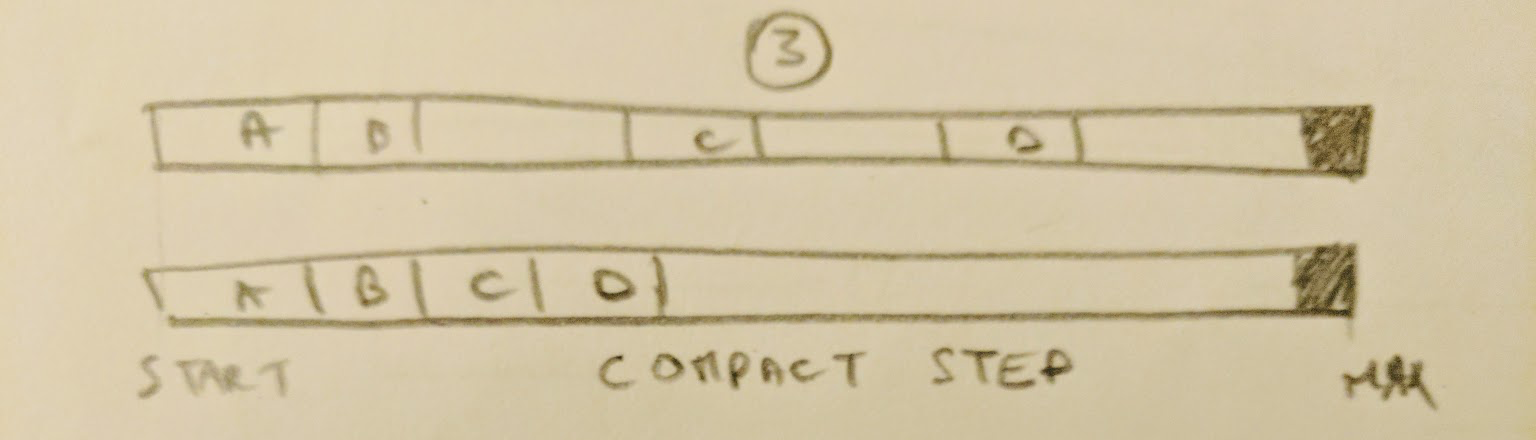
\includegraphics[width=\textwidth]{imgs/mm_compact.png}
 \end{figure}
 \par
But if memory is moved around, how do previous allocation still point to what they had before the garbage collection phase? Notice that a \cw{mmblockstruct} has a \cw{useptr} pointer which point to the owner of a block: If it moves memory, it also updates the ower of the block.

   \par
\begin{figure}[H]
\centering
 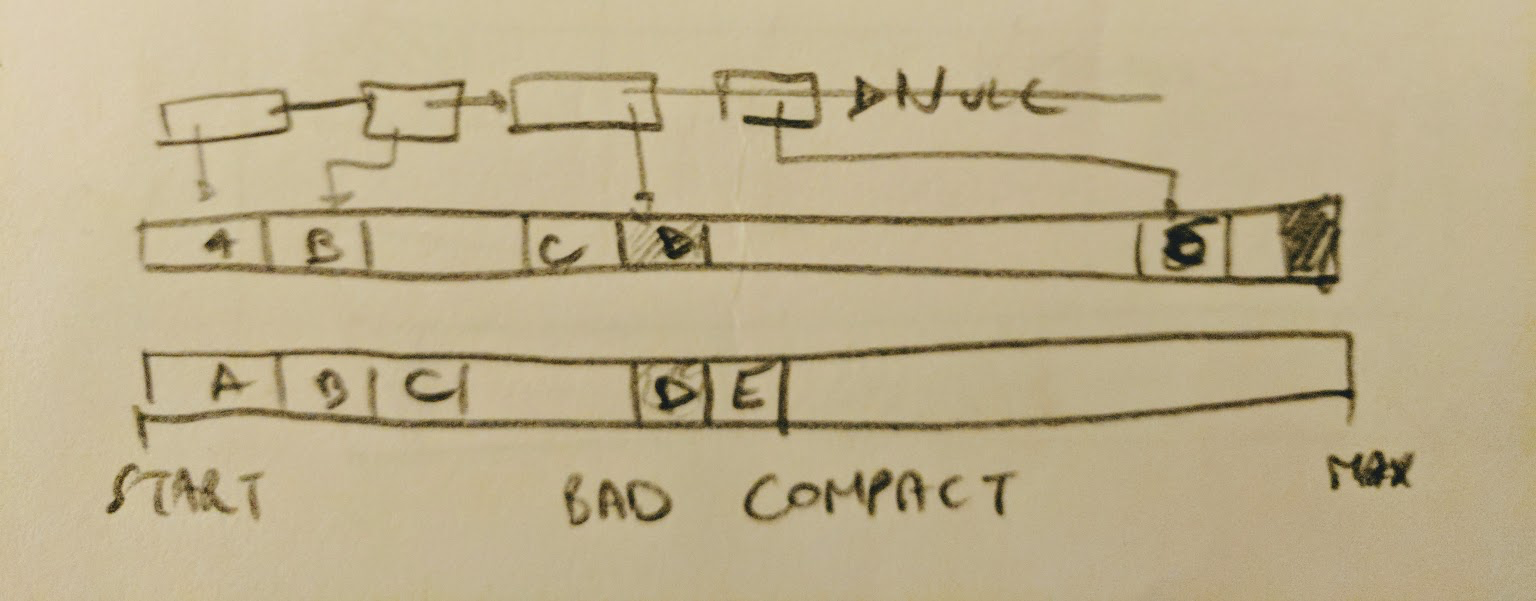
\includegraphics[width=\textwidth]{imgs/mm_compact_bad_case.png}
 \end{figure}
 \par
 Note that since some block can be marked as \cw{LOCKED}, the compacting will be disturbed: Upon encountering a locked lock, compacting start after it, even is there was space available between the last block and the locked block.












\subsection{Page Manager (PM)}
The Page Manager is dedicated to the 3D engine. Its task is to make sure assets such a wall texture, sprites and sound effect at available in RAM. Jason Blochowiak seems to be the main author and his previous experience with Unix system clearly influenced the design of this component. It is built around the idea of asset container called "Page". When the engine needs a resource, its requests a page with the resource Id to the Page Manager. To fulfill the request as fast as possible, it taps in all types of RAM: Conventional, EMS and XMS. If a page is located in conventional memory or EMS, the request is considered a cache "hit" and page is returned to caller. Otherwise the request is a cache "miss". The PM looks for the page in XMS RAM and ultimately if all failed in \cw{VSWAP.WL1} file on the HDD which contains all 3D assets.\\
 \par
\begin{figure}[H]
\centering
 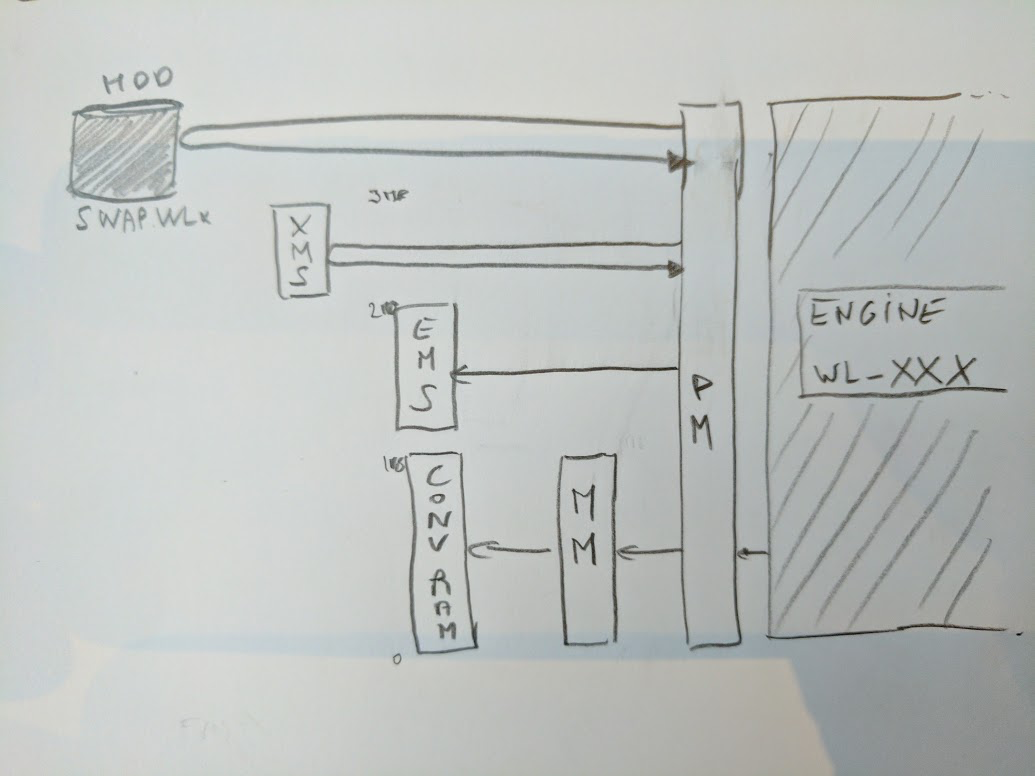
\includegraphics[width=\textwidth]{imgs/page_manager_architecture.png}
 \end{figure}
 \par
In order to minimize the cost of page miss, the engine preload the page cache before a level start. This is known at the "Get Psyched" screen:
 \par
\begin{figure}[H]
\centering
 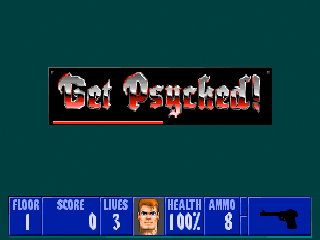
\includegraphics[width=\textwidth]{imgs/get_psyched.png}
 \end{figure}
 \par
The precaching mechanism is not particularly clever: It loads as many page from the swap file as possible. It doesn't try to look at what is actually used in the level. But the eviction policy (LRU) ultimately stabilize the cache and even a machine with only 1MB of RAM is able to play a level with no HDD access after a few minutes. This design had a small annoying flow: On a low memory machine a cache miss would occur at the worse possible moment: When the player opens the last door and is about to find himself confronted to the heavy powered final boss, the cache manager would not have the sprites available. This would incur a HDD access, a lag and an unfair death.\\
\par
The size of the swap file varies depending on the version of the game you play: \cw{VSWAP.WL1} (shareware) is 742KB while \cw{VSWAP.WL6} (full version) is 1,500KB. In both case a machine with 2MB of RAM on top of the factory issued 1MB is enough to have all assets loaded during pre-caching.\\
\par
\bu{Trivia:} In the code, the progress bar was called a "thermometer".\\
\par
\bu{Trashing:} When the system has to evict pages but ends up reloading the same resource during the same frame, it is trashing. The HDD is put to heavy contribution and the framerate drops. Trashing can happen if two many different resources are visible on the screen. In order to help designers balance their creativity with the needs for a decent framerate, the engine detects trashing and flashes the screen border red when it occurs.\\
\par
\bu{Sounds are special:} Because the sound cards are fed via a system of interrupt, the sound manager cannot recover from a page miss. Therefore all sound resources are loaded first (they are located at the start of \cw{SWAP.WL1}) and they are also only loaded in Conventional memory.











\subsection{Video Manager (VL \& VH)}
The video manager features two parts:
\begin{itemize}
\item A part dedicated to VGA register manipulation.
\item A part dedicated to 2D menu drawings.
\end{itemize}
\par
This part features what I think is one of the most beautiful trick in the game: FizzleFade which is explained later.






\subsection{Cache Manager (CA)}
A small manager performing a lot: Interface with map, graphic and music. Assets are stored in two files: One header file performing the translation between resource ID and offset in the DATA file and an other file containing he actually payload.\\
 \par
\begin{figure}[H]
\centering
 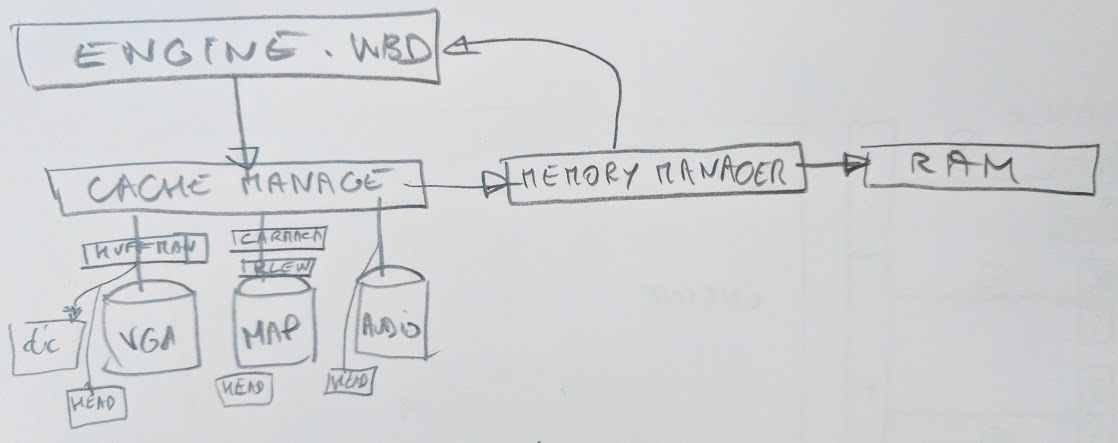
\includegraphics[width=\textwidth]{imgs/cache_manager_architecture.png}
 \end{figure}
 \par
\bu{Note:} All resources are compressed. The CM handle decompression transparently.










\subsection{User Manager (US)}
\begin{minipage}{0.7\textwidth}
Largely based on Catacom 3D code and written by Jason Blochowiak. The copy/past is very visible since 90\% of the functions declared in the header (ID\_US.H) are not actually implemented in \cw{ID\_US.C}. 
It is a poorly named manager since it takes care mostly of graphic layout. When a \cw{WL\_*} high level routines needs to draw a string, it is passed to \cw{US\_Print} which does all measurement (e.g: Draw string centered)
and then passes these information to the Video Manager (\cw{VW\_DrawPropString}) which takes care of rendition.
\end{minipage}
\begin{minipage}{0.3\textwidth}
\begin{flushright}
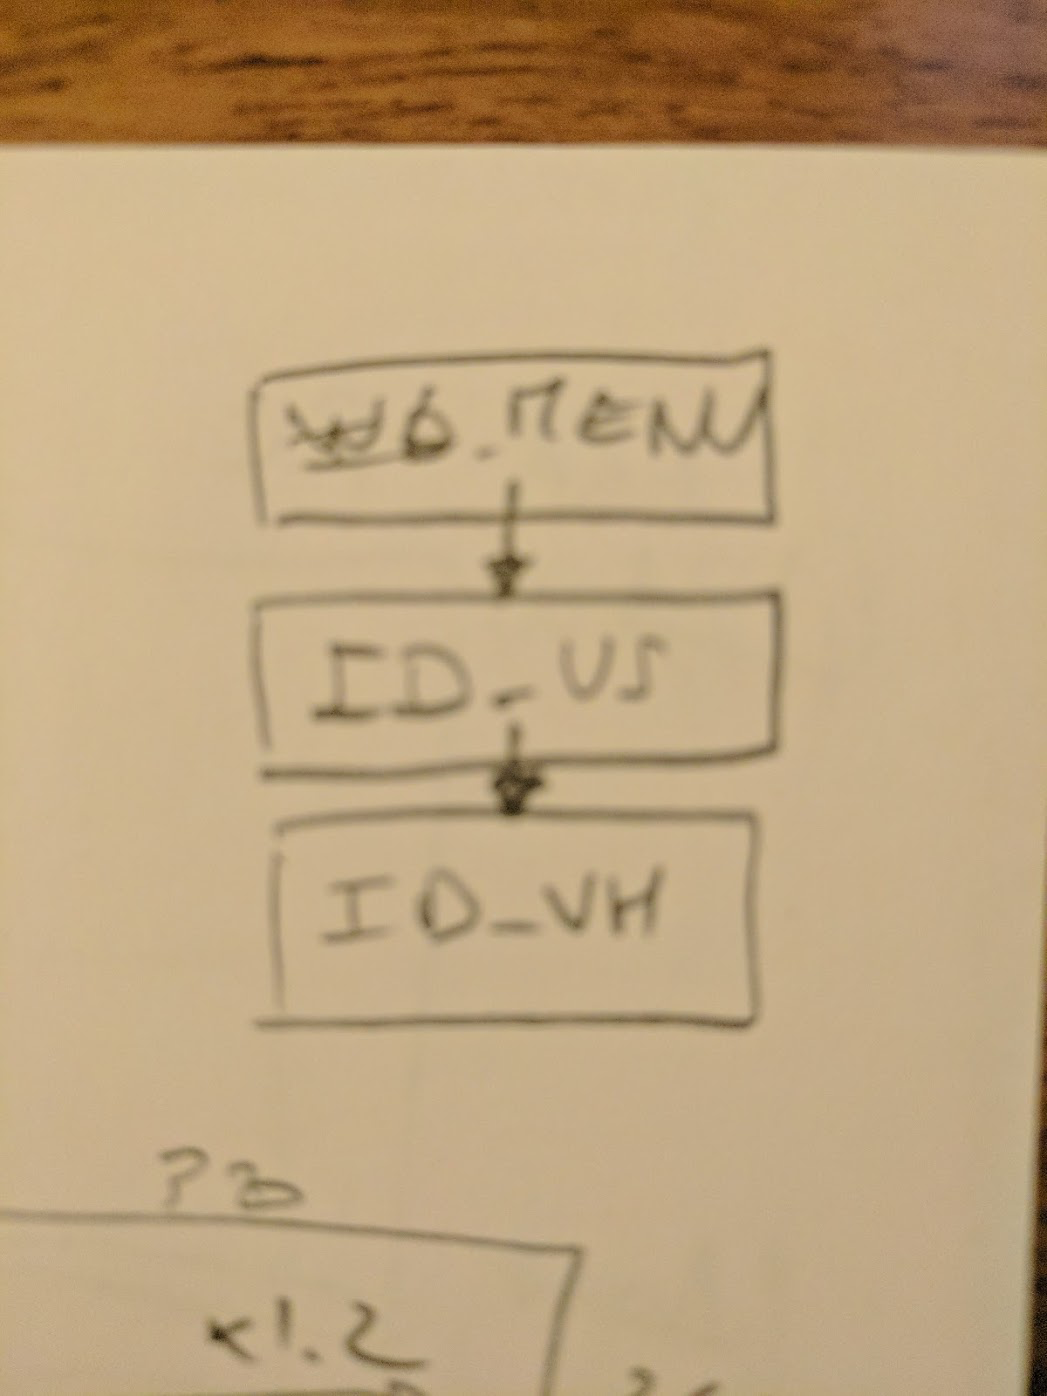
\includegraphics[width=0.8\textwidth]{imgs/US_explained.png}
\end{flushright}
\end{minipage}
\noindent
\\












\subsection{Sound Manager (SD)}
The Sound Manager abstracts interaction with all four sound systems supported: PC Speaker, ADLib (Music only), Sound Blaster and SoundSource. It is a beast of his own since it doesn't run inside the engine. Instead it called via IRQ at a much higher frequency than that engine (the engine runs at 70Hz, the sound manager ranges from 150Hz to 7000Hz). For efficiency it is written in assembly and is privileged when it comes to memory allocation: All its allocation are in Conventional Memory and its assets can never miss the cache in the Page Manager.\\
 \par
\begin{figure}[H]
\centering
 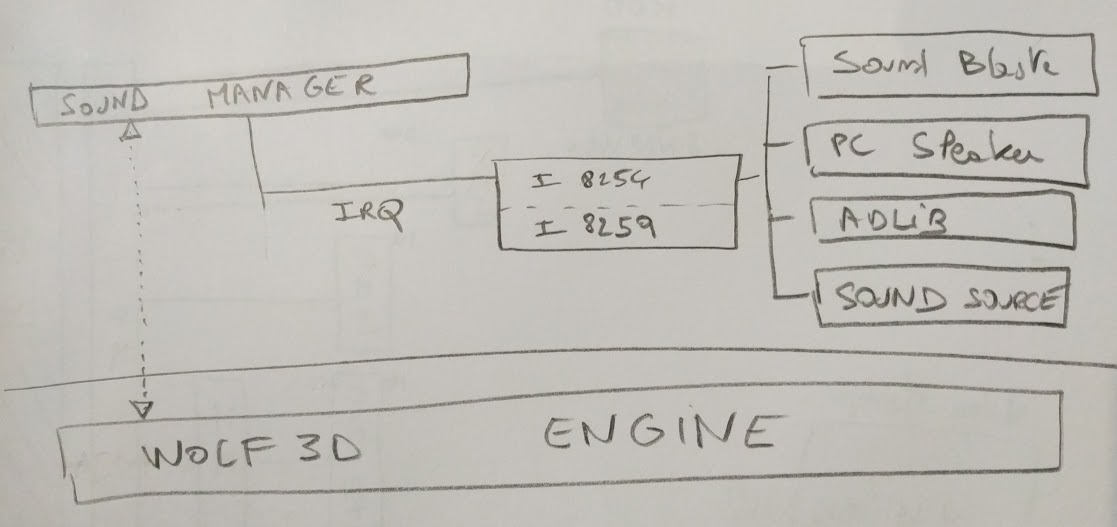
\includegraphics[width=\textwidth]{imgs/sound_manager_architecture.png}
 \end{figure}
 \par
The source manager is described extensively in the "Sound and Music" section.

















\subsection{Input Manager (IN)}
Abstract interaction with joystick keyboard and mouse. Features a lot of boring boilerplate code to deal with PS/2, Serial and DA-15 ports.























\section{Solving the VGA}\label{SetupPages}
An important problem left open in the Hardware chapter, is the video output: None of the VGA modes described in the user manual are suited for a game engine. The more important thing is to have a double buffer to avoid tearing.\\

 The most appealing one (13h) offers a single framebuffer at a resolution of 320x200 with 256 indexed colors...which is not even square pixels (the 320x200 framebuffer is stretched to 320x240 on the CRT screen). Nothing can be done about the non square pixels but luckily something that can be done about the absence of double buffering:\\
\par
 In mode 13h, the VGA circuitry automatically maps the 16K address space to the four VGA banks. It is called "chaining" and even though it wastes 75\% of the RAM it offers a linear framebuffer to the developer.\\
 \par
 Mode 13h is how the engine initialize the graphic pipeline:\\
\par
 \begin{minipage}{\textwidth}
\lstinputlisting[language=C]{code/init_vga.c}
\end{minipage}
 \par

The resulting system can be seen as follow:\\

 \par
\begin{figure}[H]
\centering
 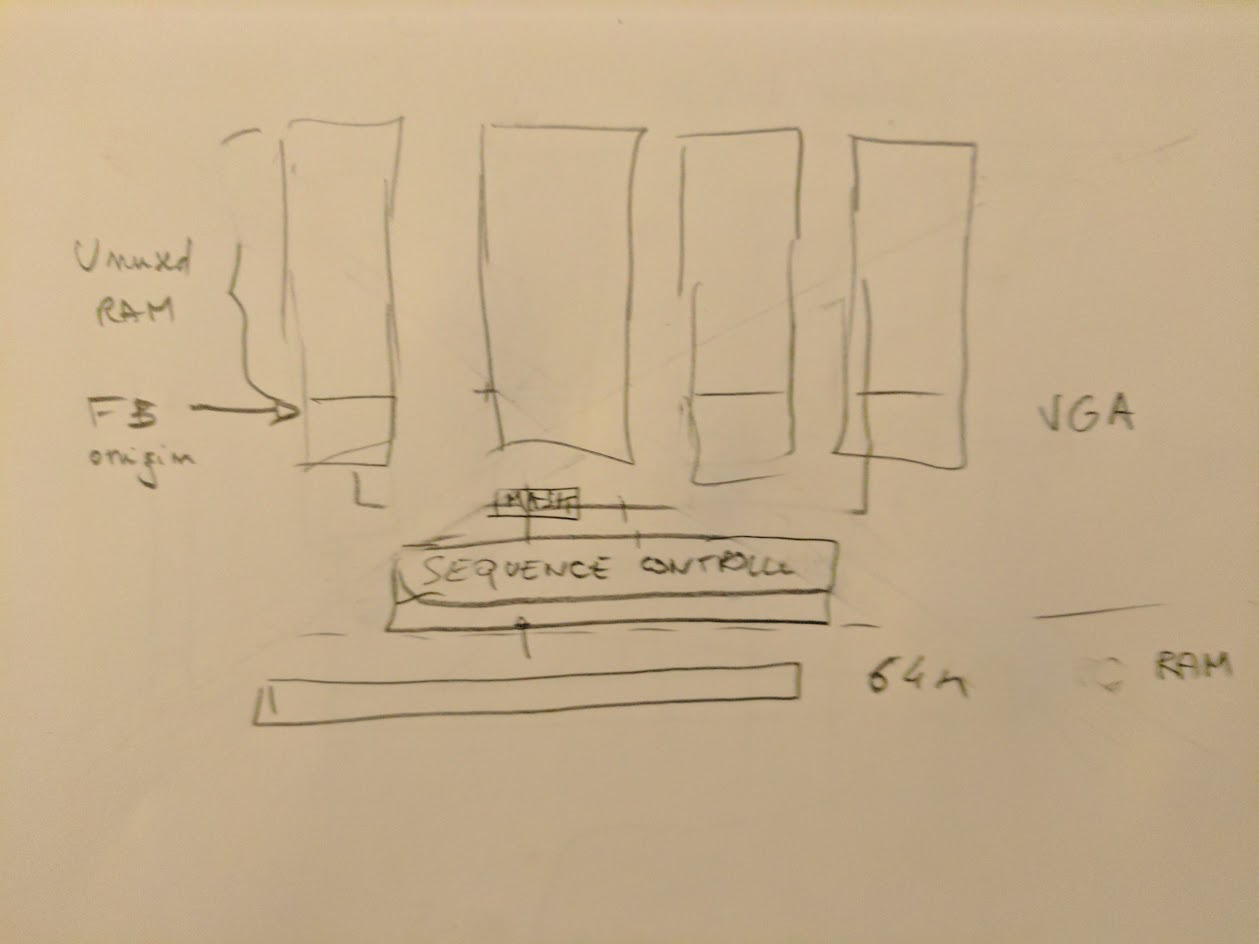
\includegraphics[width=\textwidth]{imgs/vga_layout/wasted_vga_ram.png}
 \caption{3D View as is appears on screen} \label{fig:vga_layout_in_3D}
 \end{figure}

 \par
 So the problem really is the Chain-4 chip. Even though it is undocumented there is a way to disable it. Nobody can remember who invented unchaining but it was popularized by Michael Abrash\footnote{in Dr. Dobb's Journal} in July 1991. By tweaking the VGA Sequence controller the chaining can be disabled. The developer now has to manually drive the VGA mask to plot pixel but the full 256k of ram is available. This VGA mode is commonly called "Mode X". Note: In the engine, unchaining is called "deplane" in VL\_DePlaneVGA.\\
 \par
 \begin{minipage}{\textwidth}
\lstinputlisting[language=C]{code/unchaining.c}
\end{minipage}
 \par
 To manually set the mask and select the bank were a value will be written can be done as follow:\\
 \par
 \begin{minipage}{\textwidth}
\lstinputlisting[language=C]{code/select_plan.c}
\end{minipage}
 \par
 With that much RAM available, wolf3d divides the VRAM in four parts:
 \begin{itemize}
 \item 64K for Framebuffer 0
 \item 64K for Framebuffer 1
 \item 64K for Framebuffer 1
 \item 64K for Graphic assets
\end{itemize}
\par
\begin{figure}[H]
\centering
 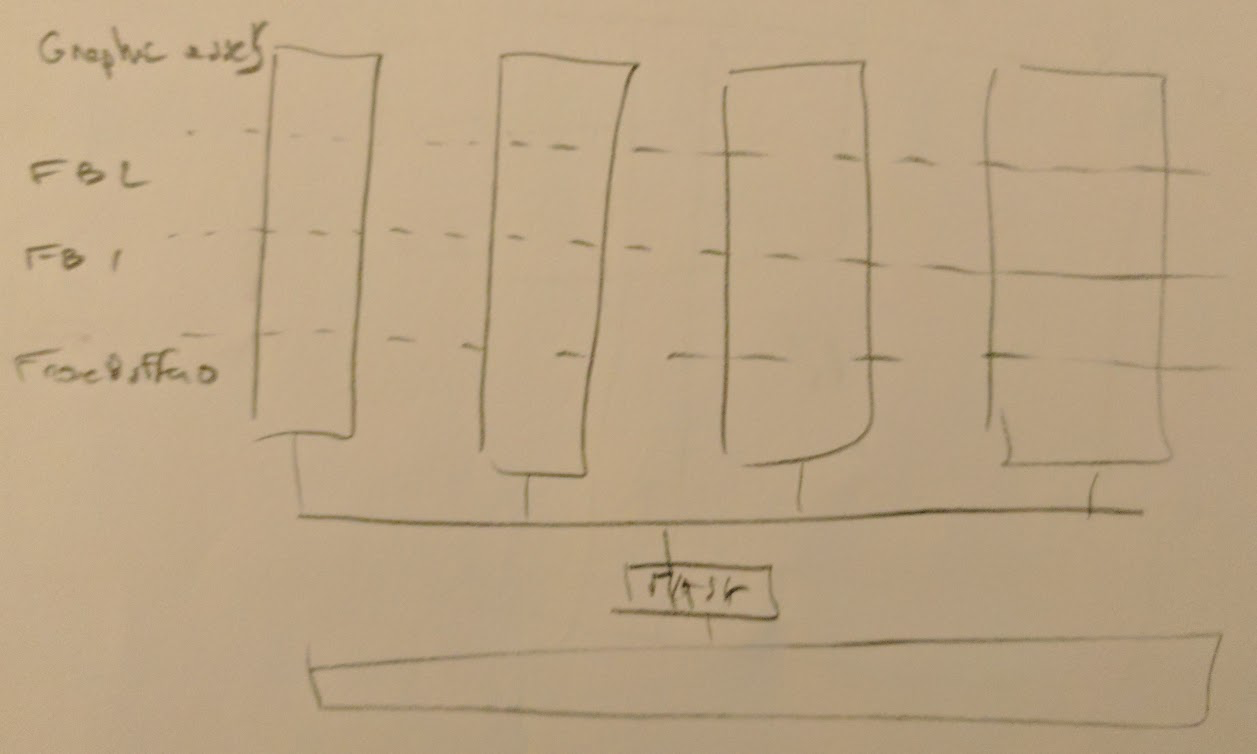
\includegraphics[width=\textwidth]{imgs/vga_layout/vga_ram_architecture.png}
 \caption{3D View as is appears on screen} \label{fig:vga_layout_in_3D}
 \end{figure}
\par
In the code it is done like this:\\
\par
 \begin{minipage}{\textwidth}
\lstinputlisting[language=C]{code/vga_setup_pages.c}
\end{minipage}
\par

Note: Why use 208 height if the framebuffer is 200 pixels tall? That doesn't make sense at first sight. I thought it was a typo (after all 0 and 8 are visually close). Think about it and find out why in section \ref{Flippingbuffer}!\\
\par


As a result from unchaining a complete framebuffer is divided into four banks. Horizontally it looks a little bit like mashed potatoes:
 \begin{figure}[H]
\centering
 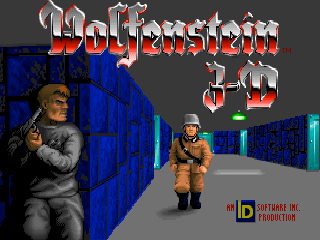
\includegraphics[width=\textwidth]{imgs/vga_layout/intro.png}
 \caption{Intro screen as it appear on screen}
 \end{figure}
 \par
 \begin{figure}[H]
\centering
 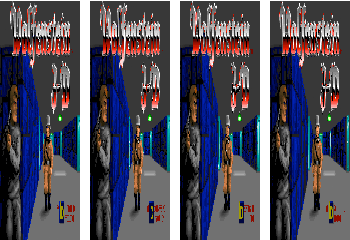
\includegraphics[width=\textwidth]{imgs/vga_layout/intro_bank.png}
 \caption{Intro screen as it is stored across 4 banks in a framebuffer} \label{fig:vga_layout_for_intro}
 \end{figure}
\par
An other example during a 3D sequence
\begin{figure}[H]
\centering
 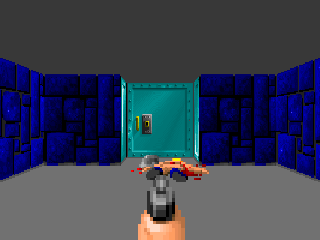
\includegraphics[width=\textwidth]{imgs/vga_layout/wolf3d_7.png}
 \caption{3D View as is appears on screen} \label{fig:vga_layout_in_3D}
 \end{figure}
 \par
 \begin{figure}[H]
\centering
 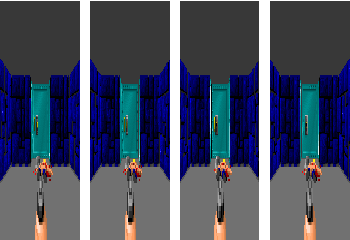
\includegraphics[width=\textwidth]{imgs/vga_layout/wolf3d_7_bank.png}
 \caption{3D View as it is stored across 4 banks in a framebuffer}
 \end{figure}

\par
But this solution only leads to an other problem. The Chain-4 chip hardwired and therefore it is fast while piloting the SC\_MASK manually via in/out BIOS operations is very VERY slow. A naive algorithm drawing left to right and top to bottom as follow could not go beyond 4-5 frames per seconds:\\
\begin{verbatim}
void CleanScreen(y, color) {
  for(int y=0 ; y < 200 ; y++) {
    for(int x=0; x < 320 ; x++) {
      selectPlan(x % 4);
      writePixel(x, y, color);   
    }
  }
}
\end{verbatim}\\
The culprit being the 320*200=64000 slow instruction to set the mask. But if we look carefully at the screenshot in Figure \ref{fig:vga_layout_for_intro} and Figure \ref{fig:vga_layout_in_3D} on page \pageref{fig:vga_layout_in_3D} there is an interesting property: If horizontal lines of pixels are broken into four areas (and it looks like mashed potatoes), vertically the column of pixesls are still linear and not broken down in banks. Indeed 320 is evenly divisible by 4 so vertically pixels are aligned and grouped in column of 80 pixels. This observation unlock a different algorithm where things are drawn vertically:\\

\begin{verbatim}
void CleanScreen(y, color) {
  for(int x=0; x < 320 ; x++) {
    selectPlan(x % 4);
    for(int y=0 ; y < 200 ; y++) {
      writePixel(x, y, color);   
    }
  }
}
\end{verbatim}\\
This code can run without issues at 70 frames per second: Only 200 slow out instruction are used.\\
\par
This VGA bank layout has a fundamental impact on the engine: To draw anything fast, it has to be drawn \underline{vertically}. This hardware constraints has deep ramification in the engine: From the algorithms picked during 2D and 3D all the way up to the assets compression techniques. In wolf3d: Everything is vertical!\\

\begin{figure}[H]
\centering
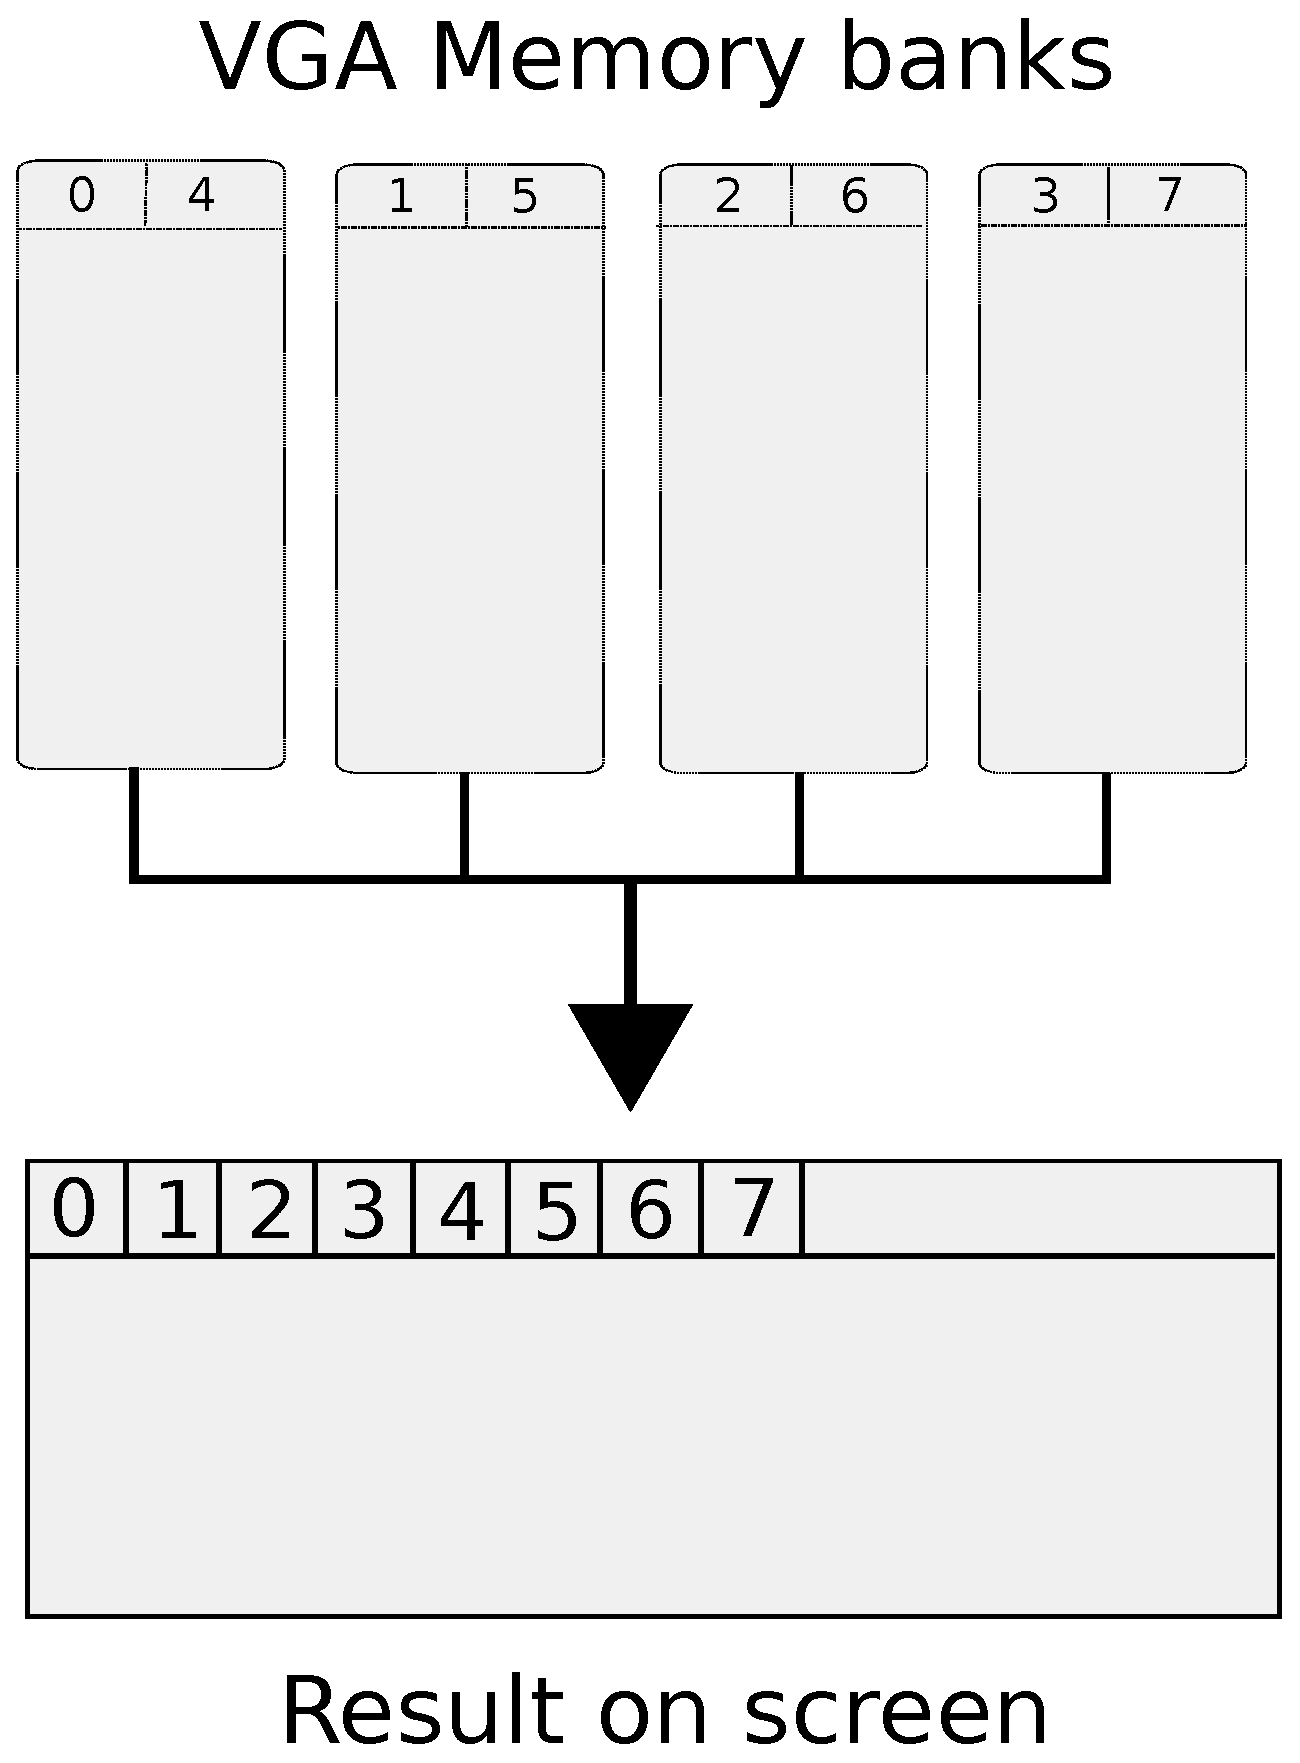
\includegraphics[width=\textwidth]{imgs/vga_ram_screen_layout.eps}
\end{figure}

Even though it was convoluted it allows clever tricks. Let's take the example of clearing the screen to black. A naive approach would be to write every pixels left to write and top to bottom:\\
\par
\begin{minipage}{\textwidth}
\lstinputlisting[language=C]{code/vga_clear/naive.c}
\end{minipage}

The cost of this operation is $320*200=64000$ writes and 64000 out operation (to select the mask).
But the overhead of selecting the bank (a.k.a plan) would make the task impossibly slow. A better approach would be to do bottom up and left to right as follow:\\
\par
\begin{minipage}{\textwidth}
\lstinputlisting[language=C]{code/vga_clear/optimized.c}
\end{minipage}

The code is slightly more complicated but this way we only switch bank XXX times and write $320*200=64000$ writes and 320 out out operation. But there is a way to do even better:\\
\par
\begin{minipage}{\textwidth}
\lstinputlisting[language=C]{code/vga_clear/optimal.c}
\end{minipage}

Which results in $320*80=25600$ and 1 out operation !\\

This is not always that easy: You can write up to four pixels in one write as long as they are properly aligned. See the example following:
\begin{figure}[H]
  \centering
 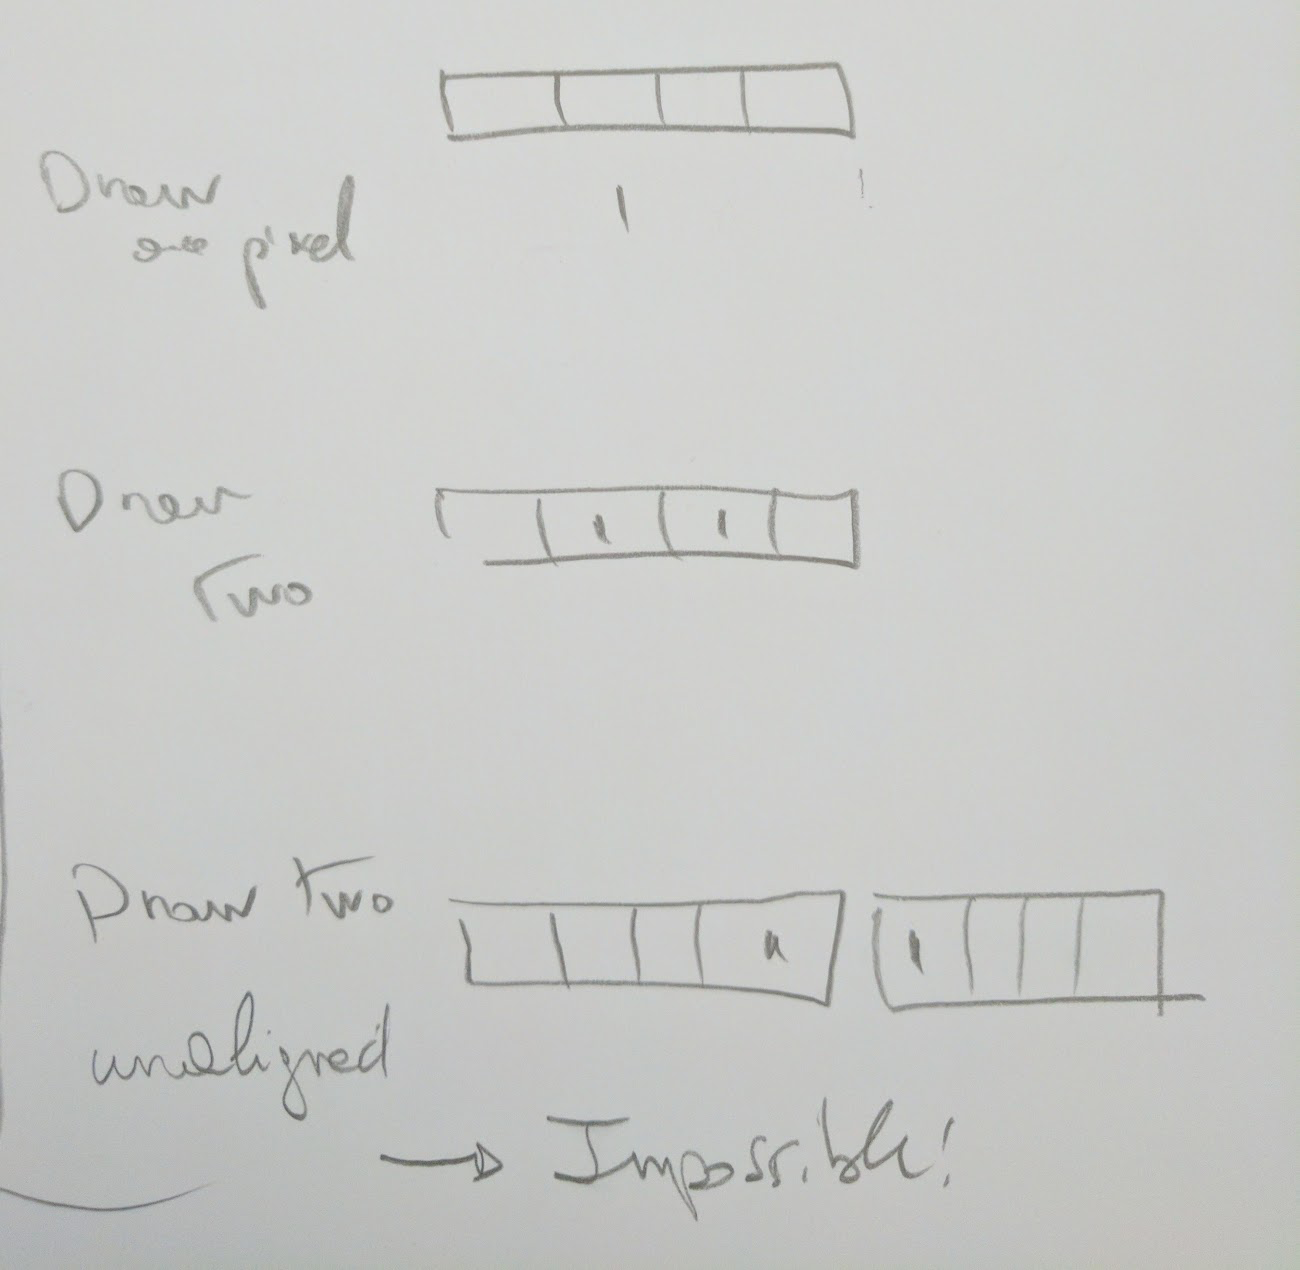
\includegraphics[width=\textwidth]{imgs//vga_multiple_pixel_write.png}
\end{figure}

\note{Ask John Carmack why they went for Mode-Y instead of Mode-X which offered square pixels.}

\par
With this technique the 64KB of mapped RAM can access the full 256KB of the VGA. This enables a mode offering:
\begin{itemize}
  \item Resolution of 320x200
  \item Double buffering
  \item Storage of sprites in VRAM.
\end{itemize}

Compared to figure 
TODO: New Drawing of VGA RAM.\\
But there is still a problem: Switching the target RAM was very slow. So a routine drawing an horizontal line on the screen:

\begin{verbatim}
void DrawLine(y, color) {
  for(int x=0; x < 320 ; x++) {
    SelectBank(x % 4);
    WritePixel(x, y, color);   
  }
}
\end{verbatim}\\
Would have been unpractical. But something else can be done if you notice that 320 is a multiple of 4 (320/4=80): If you draw only columns you don't have to change the target plan often.\\
TOOD: Drawing of how column line up in VGA RAM.\\

 \par



\subsection{Signon}
At this point, the memory manager and the vga are initialized but nothing else. In order to make player wait for the rest of system to initialize, the engine displays the famous "PG13" screen (called in the engine "signon").
\begin{figure}[H]
\centering
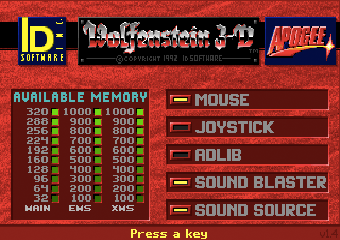
\includegraphics[width=\textwidth]{imgs/signon.png}
\caption{Architecture and sub-systems.}
\end{figure}
Since the graphic pipeline is not initialized at this point, the full 64K pg13 screen ships compiled in the executable. The engine only copies from RAM to the VGA banks.\\
\par 
\begin{minipage}{\textwidth}
\lstinputlisting[language=C]{code/signonscreen.c}
\end{minipage}
Note: In an effort to get more RAM available, these 64K are unlinked for RAM.\\
Note: The palette ($3*256=768$bytes) is also compiled in the executable. It is simply copied from RAM to VGA's DAC.
Note the main (conventional memory) which goes only up to 320K: Between the executable and other residence routines it is all what was remaining of the original 640K. The game is able to run on 320KB but you needs to swap with the HD at runtime to load textures and sprites.







\subsection{Profound Carnage}
The legendary "Profound Carnage-13" self-proclaimed rating, spoofing the movie industry PG-13 rating. Mark of the irreverent id software mindset at the time. Things like these would not fly these days.
\begin{figure}[H]
\centering

\includegraphics[width=\textwidth]{imgs/pg13.png}
\caption{Architecture and sub-systems.}
\end{figure}


\end{document}